\documentclass[
    fontsize=12pt,
    paper=a4,
    abstract=false,
    numbers=noenddot,
    listof=totoc,
    bibliography=totoc,
    %twoside,
    %open=right,
    %cleardoublepage=plain,
    parskip=half+
]{scrreprt}

\setcounter{tocdepth}{3}  % Inhaltsverzeichnis bis Subsubsection
\setcounter{secnumdepth}{3} % Nummerierung bis Subsubsection

% General stuff
\usepackage[utf8]{inputenc} % CHANGE HERE IF NECESSARY
\usepackage[T1]{fontenc}
\usepackage[ngerman]{babel} % last language given is used (here: new german)
\usepackage{lmodern}
%\usepackage{microtype}
\usepackage{ifpdf}
\usepackage{ifthen}

% Set date here 
%\day=6 \month=6 \year=2012

% Set name and title
\author{Insert your name here}
\title{Insert title here}
\date{\today}

%%%%%% %%%%%%

% Load packages ...
\usepackage{setspace}
\onehalfspacing

\usepackage{geometry}
\geometry{
    left = 4cm,
    right = 2cm,
    top = 2cm,
    bottom = 2cm,
    footskip = 7.5mm
}

\usepackage{mathptmx}
\usepackage{float}

% Corporate Design
\usepackage{eso-pic}
\usepackage{color}
% Comment out if the RUB fonts are installed
% Link: https://noc.rub.de/~jobsanzl/latex/rubtexfonts-0.4.tar.gz
%\usepackage{rubfonts2009} 
\newcommand{\setrubfontnormal}[1]{\fontfamily{rubscala}\fontsize{#1}{1}\selectfont}
\newcommand{\setrubfontextra}[1]{\fontfamily{rubflama}\fontsize{#1}{1}\selectfont}
\definecolor{rubgreen}{cmyk}{0.5,0,1,0}
\definecolor{rubblue}{cmyk}{1,0.5,0,0.6}

% Figures
\usepackage{graphicx}
\usepackage{subfig}
\usepackage{placeins}

% Tables
\usepackage{booktabs}
\usepackage{marvosym}
\usepackage{multirow}

% Math stuff and units
\usepackage{latexsym,amsmath, amssymb, amsfonts, upgreek}
\usepackage{siunitx}
\newcommand{\mathup}{\mathrm}

% Glossary
\usepackage[nonumberlist, acronym, toc]{glossaries}

% Enable quotes by \enquote{}
\usepackage[babel,english=american, german=quotes]{csquotes}

% Necessary for frontpage, allows to create automata and fancy graphics
\usepackage{tikz}

% Protocols and bytefields
% \usepackage{protocol}
\usepackage{bytefield}

% Source code listings
\newcommand{\code}[1]{\texttt{#1}}
\definecolor{colIdentifier}{rgb}{0,0,0}
\definecolor{colComments}{rgb}{0.5,0.5,0.5}
\definecolor{colKeys}{rgb}{0,0,1}
\definecolor{colString}{rgb}{0,0.6,0}

\usepackage{caption}
\usepackage{listings}
\lstset{%
	float=hbp,%
	basicstyle=\ttfamily\scriptsize, %
	identifierstyle=\color{colIdentifier}, %
	keywordstyle=\color{colKeys}, %
	stringstyle=\color{colString}, %
	commentstyle=\color{colComments}, %
	columns=flexible, %
	tabsize=2, %
	aboveskip={1.5\baselineskip}, %
	frame=single, %
	extendedchars=true, %
	showspaces=false, %
	showstringspaces=false, %
	numberstyle=\tiny, %
	breaklines=true, %
	backgroundcolor=, %
	breakautoindent=true, %
	captionpos=b%
}

% Algorithms
\usepackage[ruled, vlined, linesnumbered,algochapter,algo2e]{algorithm2e}
\renewcommand{\listalgorithmcfname}{Algorithmenverzeichnis}

% Format page foot and header
\usepackage{scrlayer-scrpage}
\clearscrheadings
\clearscrheadfoot
\automark[section]{chapter}
\cfoot{\pagemark}
\renewcommand*{\chapterpagestyle}{scrheadings}
\pagestyle{scrheadings}

%% use some standards for mathematical expressions:
\newcommand{\red}{{\rm red}}
\newtheorem{theorem}{Theorem}[section]
\newtheorem{lemma}[theorem]{Lemma}
\newtheorem{proposition}[theorem]{Proposition}
\newtheorem{corollary}[theorem]{Corollary}
% \newtheorem{definition}[theorem]{Definition}
\newtheorem{algorithm}[theorem]{Algorithm}
\newenvironment{example}{\begin{quote}{\bf Example:}}{\end{quote}}

% BIBTEX, http://mirrors.ctan.org/biblio/bibtex/contrib/babelbib/babelbib.pdf
\usepackage{babelbib}
\usepackage{url}
\def\UrlBreaks{\do\/\do-}

% \setbibpreamble{{\large Seitenzahlen, auf denen ein Eintrag referenziert wird, werden am Ende eines jeden Eintrags angegeben.}\newline} % Wegen der pagebackref-Option des hyperref-Packets, wird vielen nicht direkt klar was das soll http://projekte.dante.de/DanteFAQ/Verzeichnisse#16

% gray definition boxes, that whay you'll find them in the text
\usepackage{shadethm}
\newshadetheorem{sthm}[figure]{Definition}
\newenvironment{definition}[1][]{
   \definecolor{shadethmcolor}{rgb}{.9,.9,.9}
   \begin{sthm}[#1]
 }{\end{sthm}}

% experimental
%\usepackage{scrhack}

% Hyperlinks and menu for your document
\usepackage[breaklinks,hyperindex,colorlinks,anchorcolor=black,citecolor=black,filecolor=black,linkcolor=black,menucolor=black,urlcolor=black,pdftex]{hyperref} % pagebackref: Add page number to the references where they can be found
% DO NOT LOAD ANY OF YOUR PACKAGES BEYOND THIS PACKAGE

\makeatletter
\AtBeginDocument{
 \hypersetup{
   pdftitle = {\@title},
   pdfauthor = {\@author},
   pdfsubject={\@title},
   pdfkeywords={SAML, add more}, % CHANGE HERE
%    unicode={true},
 }
}
\makeatother

% Use the same counter for tables and figures
\makeatletter
\AtBeginDocument{
\let\c@table\c@figure
\let\c@lstlisting\c@table
\let\c@algocf\c@lstlisting
}
\makeatother

\ifpdf
	\hypersetup{linktocpage=false} 	% false=links are section names, true=links are page numbers, IMPORTANT: in dvi2ps mode, 'true' is required!
\else
	\hypersetup{linktocpage=true} 		% false=links are section names, true=links are page numbers, IMPORTANT: in dvi2ps mode, 'true' is required!
	\usepackage[hyphenbreaks]{breakurl}
\fi


\begin{document}

    \clearpage
%\pagestyle{scrheadings}
\tableofcontents
\clearpage

    \pagenumbering{arabic}
\setcounter{page}{3}
\chapter{Einführung} % erster Überblick über Programmiersprachen insgesamt
Programmiersprachen sind aus der modernen Zeit des 21. Jahrhunderts kaum noch wegzudenken, weil sie für alle elektronischen Geräte gebraucht werden. Mithilfe von Programmiersprachen werden dem Computer Algorithmen, welche Abfolgen von Befehlen und Rechnungen sind, mitgeteilt\cite{Louis:2010}. Laut \cite{Louis:2010} übersetzt ein Compiler die Programmiersprache in Maschinencode, welcher von der \textit{Central Processing Unit} (CPU) verstanden wird. Das Übersetzen von Programmiersprachen in Maschinencode erleichtert die Arbeit für Programmierer ungemein, da Programmiersprachen für den Programmierer intuitiver, verständlicher, übersichtlicher und naheliegender sind als Maschinencode. Grace Hopper hat den ersten Compiler 1952 entwickelt und gilt somit als eine Pionierin der Programmierung.


\par % Wieso Python und wieso Java
Über die Zeit haben einige Programmiersprachen besonders an Bedeutung gewonnen. 
Zwei Programmiersprachen, die viel Beliebtheit genießen, sind Java und Python. 
Java wird unter anderem am Nepomucenum Coesfeld zum jetzigen Zeitpunkt im Informatik-Unterricht der Jahrgangsstufe Q1 unterrichtet. 
Die Popularität von Python steigt Jahr für Jahr, da Python gerne für künstliche Intelligenz und \textit{Deep Learning} genutzt wird, mit der steigenden Nachfrage nach künstlicher Intelligenz \cite{Github:PYPL}\cite{Gray:2017}. 
Python hat Java 2018 als beliebteste Programmiersprache abgelöst.
Es ist folglich vorteilhaft ein Grundwissen von Prinzipien und Syntax von Python zu haben. 

\par % was wird mit Python gemacht und wieso nicht mit Java. Warum ist es wichtig Python zu können.
Python wird im Rahmen dieser Facharbeit für die Implementierung eines hexagonalen Schachs praktisch angewandt. 
Auf eine gegenüberstellende Implementierung des hexagonalen Schachs mit Java wird verzichtet, da dies zu umfangreich für die Facharbeit wäre. 
Ein besseres Verständnis wird durch Vorkenntnisse in der Programmiersprache Java und/oder Python ermöglicht, ist jedoch nicht essenziell. 

\par % woher kommt die Idee des hexagonalen Schachs
Die Idee zum Implementieren eines hexagonalen Schachs, um die Programmiersprache Python in einem praktischen Beispiel zu evaluieren, rührt von dem Video "Hexagons are the Bestagons"\ von GCP Grey \cite{Grey:Bestagons}. 
In diesem wird erst ausführlich erörtert, weshalb das Hexagon die beste Form ist und danach wird hexagonales Schach als Beispiel für Spiele genannt, welche von einer hexagonalen Abwandlung profitieren würden.

    \newacronym{ide}{IDE}{Intelligent Development Environment}

\chapter{Grundlagen}

Java ist eine objektorientierte, kompilierte Programmiersprache, welche plattformunabhängig ist. Sie wurde von der Programmiersprache C inspiriert, weshalb Java eine ähnliche Syntax hat. Java erschien 1995 und wird jeher für viele unterschiedliche Dinge genutzt. Auf der Internetseite von Oracle wird geschrieben: „Mit Java können Sie Online-Spiele spielen, mit Menschen auf der ganzen Welt chatten, Ihre Hypothekenzinsen berechnen und Bilder in 3D betrachten, um nur einige Beispiele zu nennen“\cite{Oracle:Java}. Dazu ist Java auf 13 Milliarden Geräten vertreten, und über 20 Jahre unter den drei meistgenutzten Programmiersprachen der Welt \cite{Github:PYPL}. \cite{Louis:2010}\cite{Oracle:Twitter} \par
Python wurde in den 90er Jahren von Guido van Rossum entwickelt. Er war an der Entwicklung von ABC beteiligt und hat mit der positiven und negativen Kritik Python entwickelt. Ursprünglich war sie als Skriptsprache für Amoeba gedacht. Der Name von für die Programmiersprache kommt von den britischen Komikern \textit{Monty Python}. Python ist, wie Java, ebenfalls eine objektorientierte, plattformunabhängige, interpretierte High-Level Programmiersprache. Wie ABC soll Python einfach zu verstehen und zu lesen sein. Bei Python wurde stark darauf geachtet, dass die Programmiersprache mächtig ist, was bei ABC nicht der Fall war und oft kritisiert wurde. Mit kleinen und übersichtlichen Programmen ist man in der Lage komplexe Aufgaben zu lösen. Python kann für die Web- und App-Entwicklung genutzt werden. Durch die Unmengen an Bibliotheken ist die Programmierung in Python bei neuen Themen wie künstlicher Intelligenz, Maschine Learning und Deep Learning besonders beliebt \cite{PythonCS}. Das liegt auch daran, dass Python Bibliotheken so einfach wie möglich bereitstellt. Die Standartbibliothek ist sehr umfangreich. Beispielsweise das Summieren jedes Elementes eines Arrays wird in Python mit einer einfachen Methode gemacht, während bei Java auf komplexere Wege zurückgegriffen werden muss. \cite{Python3:Buch}

\section{Grundbausteine und Funktionen}

Für den ausführlichen Vergleich der beiden Programmiersprachen, werden Syntax, Codelänge, Arbeitsspeicherauslastung und Laufzeit verglichen und daraus ein Resultat gezogen.
In Java wird der Einstiegspunkt durch das \textit{\acrlong{ide}} (IDE) BlueJ definiert. Der Startpunkt für das Programm wird von IDE zu IDE unterschiedlich definiert. Die IDE \textit{pyCharm}, welche die fünft meistgenutzte IDE der Welt ist, führt entweder eine \textit{main.py} Datei aus oder es wird manuell ein Einstiegspunkt definiert \cite{Github:IDE}. Das geschieht wie in \ref{lst:pystart} gezeigt.

\begin{lstlisting}[language=python,caption={Einstiegspunkt Python},captionpos=b,label={lst:pystart}]
if __name__ == '__main__':
\end{lstlisting}

Der Code wird eingerückt geschrieben. Der Einstiegspunkt ist nicht in einer Klasse enthalten. Wird das Programm bei einem manuellen Einstiegspunkt gestartet, wird alles Eingerückte ausgeführt, bis es unterbrochen wird. Wenn die \textit{main.py} durchlaufen wird, läuft das Dokument von oben bis unten durch. Klassen und Methoden werden beim Durchlaufen ignoriert. Dadurch wird keine Klasse gebraucht und kleine Programme können schnell programmiert werden. Eine Klasse ist ein Entwurf mit Eigenschaften und Funktionen \cite{gfg}. In Java ist eine Klasse zum Ausführen des Programms essenziell und deswegen werden als erstes die Unterschiede von Klassen gegenübergestellt.

\begin{lstlisting}[language=java,caption={Klasse in Java},captionpos=b,label={lst:java:class}]
public class Tisch
{
    public Tisch()
    {
        System.out.println("Tisch");
    }
}
\end{lstlisting}

\begin{lstlisting}[language=python,caption={Klasse in Python},captionpos=b,label={lst:python:class}]
class Tisch:
    def __init__(self):
        print('Tisch')
\end{lstlisting}

Lisiting \ref{lst:java:class} und Listing \ref{lst:python:class} schreiben, sobald sie initialisiert werden, „Tisch“ in die Konsole. Bei dieser direkten Gegenüberstellung der beiden Klassen fallen einige Unterschiede in der Syntax auf. Eine Klasse in Python wird nicht als \textit{public} oder \textit{private} definiert, sondern ist immer public. In der Klasse ist ein Konstruktor enthalten. Dieser wird unter den gleichen Bedingungen aufgerufen wie bei Java. Der Konstruktor besteht jeweils aus einem Kopf und einen Rumpf. Der Kopf in Java besteht aus dem Schlüsselbegriff \textit{public} oder \textit{private}, dem Namen der Klasse und Parameterklammern. Anders ist das in Python, wo der Konstruktor aus den Schlüsselbegriffen \textit{def} und \textit{\_\_init\_\_}, sowie den Parameterklammer und einem Doppelpunkt besteht. Der Code im Konstruktor wird beim Initialisieren der Klasse ausgeführt. Der Code endet in Java mit einem Semikolon und in Python nicht. Besonders durch die fehlenden geschweiften Klammern, sondern dem Definieren der Rümpfe durch das Einrücken des Codes ist Python um vier Zeilen kürzer. Sofern man sich an die Formatierungsregeln hält. Aber weniger Zeichen hat Python auch. Java braucht für den Code 60 Zeichen, während in Python nur 44 gebraucht werden. \par

Ein Tisch hat verschiedene Attribute. Darunter fallen Länge, Breite, Höhe, Anzahl der Beine und Dicke des Tisches. Diese Werte werden in der \textit{Random-Access Memory} (RAM) gespeichert \cite{Louis:2010}. Eine Variable hält entweder einen Wert (primitiv) oder eine Referenz auf den Wert (Referenz). Folglich ist eine Variable ein Speicherplatz. Der Wert im Speicher kann immer wieder geändert werden. In Java müssen die Werte immer mit dem Typ übereinstimmen. Java hat vier primitive Datentypen. \textit{Int, double, char und boolean} müssen immer einen Wert haben. \textit{String} hingegen greift über eine Referenz auf den Wert zu und kann deswegen auch \textit{Null} sein. Python hat keine Datentypen. Eine Variable kann immer jede Art von Wert speichern. Wie in jeder Sprache haben auch Programmiersprachen eine Art Rechtschreibung. Variablen werden nach bestimmten Richtlinien benannt, ein leichteres Lesen des Codes ermöglichen. Nach diesen \textit{naming conventions} werden Variablen in Java nach \textit{lowerCamelCase} benannt \cite{Microsoft:CapCon}. Auch die \textit{naming convention} ist in Python anders. Bei der Benennung von Variablen wird sich an \textit{snake\_case} gehalten \cite{Ims:h-s}. \cite{JavaNC}\cite{PythonStyle}\cite{JVMS}

\begin{lstlisting}[language=java,caption={Variablen in Java},captionpos=b,label={lst:java:variablen}]
public class Tisch
{
    int laenge;
    int breite = 50;
    int hoehe = 80;
    
    public Tisch()
    {
        laenge = 100;
        System.out.println("Tisch");
    }
}
\end{lstlisting}

\begin{lstlisting}[language=python,caption={Variablen in Python},captionpos=b,label={lst:python:variablen}]
class Tisch:
    def __init__(self):
        self.laenge = 100
        self.breite = 50
        self.hoehe = 80
        print('Tisch')
\end{lstlisting}

Durch die Gegenüberstellung beider Versionen mit Variablen fallen einige Dinge auf. Die globalen Variablen werden im Konstruktor initialisiert und deklariert. Das \textit{self.} macht die Variablen global. Ohne das \textit{self.} sind die Variablen nur im Konstruktor nutzbar. Variablen die nur im Konstruktor oder in Methoden nutzbar sind werden auch temporäre Variablen genannt, da der Wert nur temporär ist und nach dem Konstruktor oder der Methode verworfen wird. Soll die Variable in anderen Codeteilen aufgerufen werden, muss in Java nur den Variablenname geschrieben werden, bei Python muss das \textit{self.} davor. \par
Durch das Angeben eines Datentypens in Java, werden in Python weniger Zeichen für die Initialisierung und Deklarierung von Variablen gebraucht. Die Unabhängigkeit von Datentypen in Python ist ein großer Vorteil gegenüber Java.\par
Ein Sonderfall ist der Array oder auch die Liste. Während Java die beiden einzeln sieht, kombiniert Python die beiden. Ein Array ist eine Sammlung von Speichern für Werte mit einer konstanten Länge. Eine Liste ist eine Sammlung mit flexibler Länge, es können also Werte entfernt werden und hinzugefügt werden. Bei einem Array kann mit einem Index auf den Speicher zugegriffen werden. Eine Liste ist eine Verkettung von Werten und es kann immer nur auf das nächste Element zugegriffen werden. Wenn man auf das fünfte Element des Arrays zugreifen möchte geht das per genullten Index. Bei einer Liste wird mit dem ersten Element angefangen und es wird bis zum fünften Element auf den Nachbarn zugegriffen. Deshalb kann auch immer nur mit dem jetzigen Element in einer Liste gearbeitet werden. \cite{NRWListe}\cite{Louis:2010}\cite{Python3:Buch}

\begin{lstlisting}[language=java,caption={Array in Java},captionpos=b,label={lst:java:array}]
public class Tisch
{
    int breite;
    int laenge = 100;
  
    String[] gegenstaende = new String[3];
  
    public Tisch()
    {
        breite = 50;
    
        gegenstaende[0] = "Buch";
        gegenstaende[1] = "Stift";
        gegenstaende[2] = "Pflanze";
    }
}
\end{lstlisting}

In Java wird auf die einzelnen Speicher per Index zugegriffen, wie Listing \ref{lst:java:array} zeigt. Nachteil davon ist, dass nicht auf Index 3 zugegriffen werden kann, dieser existiert nämlich nicht. Der Array hat eine konstante Länge, welche sich nicht mehr nach der Deklarierung ändern lässt. Alle drei Elemente sind auf dem Tisch und die Anzahl der Elemente lässt sich nicht mehr verändern.

\begin{lstlisting}[language=java,caption={Liste in Java},captionpos=b,label={lst:java:liste}]
public class Tisch
{
    int breite;
    int laenge = 100;
  
    String[] gegenstaende = new String[3];
  
    public Tisch()
    {
        breite = 50;
    
        gegenstaende.append("Buch");
        gegenstaende.append("Stift");
        gegenstaende.append("Pflanze");
    }
}
\end{lstlisting}

Die Liste ermöglicht ein Hinzufügen von Elementen per \textit{append} und ein Löschen per \textit{remove}. Entfernt werden kann aber immer nur das aktuelle Element. Es lässt sich nicht per Index auf die Elemente zugreifen.

\begin{lstlisting}[language=python,caption={Liste in Python},captionpos=b,label={lst:python:liste}]
class Tisch:
  def __init__(self):
    self.laenge = 100
    self.breite = 50
    self.gegenstaende = []
    self.gegenstaende.add('Buch')
    self.gegenstaende[0] = 'Faus'
    self.gegenstaende.add('Stift')
    self.gegenstaende.add('Pflanze')
    self.gegenstaende.remove('Pflanze')
    self.gegenstaende.pop(1)
\end{lstlisting}

Python erlaubt es mit dem \textit{add()} Befehl neue Elemente der Liste hinzuzufügen. Löschen funktioniert genauso gut. Entweder per \textit{pop()}, wo in den Parameterklammern ein Basis Null Index mitgegeben wird oder mit der Funktion \textit{remove()}. \textit{remove()} arbeitet mit einem Wert anstelle eines Indexes, welcher gelöscht werden soll. Von einer Liste mit zweimal dem gleichen Wert wird das erste Element gelöscht. Das Python in der Lage ist per Index auf die Elemente zuzugreifen erleichtert das Schreiben des Codes.\par
Das Erstellen eines Arrays in Java und der Liste in Python auf diese Art und Weise kann je nach Situation umständlich sein. Deshalb bieten beide Programmiersprachen eine vereinfachte Deklaration.\newpage

\begin{lstlisting}[language=java,caption={Einfache Deklarierung eines Arrays in Java},captionpos=b,label={lst:java:ezarray}]
String[] gegenstaende = {
    "Buch", "Stift", "Pflanze"
};
\end{lstlisting}

\begin{lstlisting}[language=python,caption={Einfach Deklarierung eines Arrays in Python},captionpos=b,label={lst:python:ezarray}]
gegenstaende = [
    'Buch', 'Stift', 'Pflnaze'
]
\end{lstlisting}

Dazu kommen noch weitere Funktionen für Listen von Python, welche weder in Arrays noch in den Listen von Java enthalten sind. Beispielsweise kann man anstelle eines Indexes auch einen Bereich. Das macht Python noch kürzer und übersichtlicher\par
Methoden sind Abfolgen von Anweisungen, welche per Methodenname aufgerufen werden können. Durch das Auskapseln von Code in Methoden entstehen mehrere Vorteile. Der Code lässt sich leichter wiederverwenden, das Programm ist insgesamt strukturierter und der geschriebene Code ist verständlicher. \cite{Python3:Buch}\cite{Louis:2010}

\begin{lstlisting}[language=java,caption={Methoden in Java},captionpos=b,label={lst:java:methode}]
public void verstelleTisch(double wert)
{
    hoehe = hoehe + wert;
}
\end{lstlisting}

\begin{lstlisting}[language=python,caption={Methode in Python},captionpos=b,label={lst:python:methode}]
def verstelle_tisch(wert):
    hoehe = hoehe + wert
\end{lstlisting}

Methoden in Python haben keinen Zugriffstypen, genauso wie bei Variablen sind Methoden immer \textit{public}. Da Python keine Datentypen hat haben Methoden auch keine Rückgabewerte. Der Methodenkopf besteht nur aus dem Schlüsselbegriff \textit{def}, dem Namen und Parametern, welche von Klammern umrahmt werden. Der Rumpf der Methode wird anders als in Java nur durch das Einrücken des Codes und dem Doppelpunkt am Ende des Methodenkopfes definiert. Wird der Code nicht eingerückt geschrieben wird er nicht der Methode zugeordnet. Parameter funktionieren in Java und Python gleich. Sie werden ebenfalls nicht mit einem Datentyp angegeben. Einen Wert von einer Methode zurück zu geben ist ebenfalls möglich. Der Rückgabewert kann bei Python vom Datentyp variieren, da die Methode nicht auf einen Datentyp festgelegt ist. Java lässt unterschiedliche Rückgabewerte in der gleichen Methode nicht zu. Laut der \textit{naming convention} werden Methoden nach den gleichen Prinzipen wie Variablen genannt \cite{Ims:h-s}\cite{Microsoft:CapCon}. \cite{Python3:Buch}\cite{Louis:2010}\par
Methoden können in Python nicht überladen werden. Dafür gibt es Standartparameter. Im Methodenkopf wird dem Parameter mit dem Gleichheitszeichen ein Wert zugewiesen

\begin{lstlisting}[language=python,caption={Methode in Python mit Standartparameter},captionpos=b,label={lst:python:sparameter}]
def methode(parameter = 'standartparameter'):
    print(parameter)
\end{lstlisting}

Beim Aufrufen der in Listing \ref{lst:python:sparameter} dargestellten Methode ist ein Parameter optional. Der Wert von \textit{parameter} ist “standartparameter“ wenn kein Wert angegeben wird. Wenn ein Wert angegeben wird, wird der Wert überschrieben.
Mit der jetzigen Methode \textit{verstelleTisch} kann die Höhe beliebt sein. Das kann mit einer If-Abfrage verhindert werden. If-Abfragen sind in der Lage zwischen verschieden Fällen zu unterscheiden. In diesem spezifischen Beispiel gibt es zwei Fälle. Entweder geht die neue Höhe außerhalb des Toleranzbereichs oder sie bleibt drin. Die If-Abfrage wird in Java und Python gleich strukturiert, die Syntax unterscheidet sich jedoch. \cite{Python3:Buch}\cite{Louis:2010}

\begin{lstlisting}[language=java,caption={If-Abfrage in Java},captionpos=b,label={lst:java:if}]
if (hoehe + wert < maxHoehe && hoehe + wert > minHoehe)
{
    hoehe = hoehe + wert;
}
\end{lstlisting}

\begin{lstlisting}[language=python,caption={If-Abfrage in Python},captionpos=b,label={lst:python:if}]
if hoehe + wert < maxHoehe && hoehe + wert > minHoehe:
    hoehe = hoehe + wert;
\end{lstlisting}

Listing \ref{lst:python:if} zeigt, dass der Doppelpunkt am Ende des Kopfes, sowie das Einrücken den Rumpf definieren.
Trotz der Ähnlichen Operatoren unterscheiden sich Python und Java bei den essenziellen Operatoren. \textit{\&\&} und \textit{||} werden in Python zu \textit{and} und \textit{or}. Die Funktionsweise bleibt gleich. Ebenfalls wichtig ist, dass das \textit{!} zu einem \textit{not} wird. Mit \textit{not} lassen sich genauso wie in Java \textit{boolean}-Werte umdrehen. \textit{Is} wird genutzt, um eine Variable mit \textit{None} zu vergleichen. Kombiniert mit \textit{not}, gibt \textit{is not} den Wert gedreht zurück. \cite{Python3:Buch}\cite{Louis:2010}
Die dazugehörigen \textit{else if} und \textit{else} Zweige gibt es in Python ebenfalls. Lediglich wird \textit{else if} zu \textit{elif}. Durch die Operatoren wird deutlich das Python besser zu lesen ist. Die Längen der If-Abfragen unterscheiden sich unwichtig minimal.\par
Als letztes werden die Schleifen in Java und Python gegenübergestellt. Schleifen wiederholen Aktionen solange bis eine Bedingung erfüllt ist. Dazu wird entweder die \textit{while}-Schleife oder die \textit{for}-Schleife genutzt.

\begin{minipage}{.5\linewidth}
\begin{lstlisting}[language=java,caption={while-Schleife Java},captionpos=b,label={lst:java:while},numbers=left, frame=none]
String[] gegenstaende = {
    "Buch", "Stift", "Pflanze"
};

public void schreibeGegenstaende()
{
    int i = 0;
    while (i < gegenstaende.length())
    {
        System.out.println(Gegenstaende[i]);
        i++;
    }
}
\end{lstlisting}
\end{minipage}
\begin{minipage}{.5\linewidth}
\begin{lstlisting}[language=python,caption={while-Schleife Python},captionpos=b,label={lst:python:while},frame=l]
gegenstaende = [
    'Buch', 'Stift', 'Pflanze'
]

def schreibe_gegenstaende():
    i = 0
    while i < range(len(gegenstaende)):
        print(gegenstaende[i])
        i += 1
        
        

.
\end{lstlisting}
\end{minipage}

\begin{minipage}{.5\linewidth}
\begin{lstlisting}[language=java,caption={for-Schleife Java},captionpos=b,label={lst:java:for},numbers=left, frame=none]
public void schreibeGegenstaende()
{
    for(int i = 0; i < gegenstaende.length(); i++)
    {
        System.out.println(gegenstaende[i]);
    }
}
\end{lstlisting}
\end{minipage}
\begin{minipage}{.5\linewidth}
\begin{lstlisting}[language=python,caption={for-Schleife Python},captionpos=b,label={lst:python:for},frame=l]
def schreibe_gegenstaende():
    for i in range(len(gegenstaende)):
        print(gegenstaende[i])
        
        

.
\end{lstlisting}
\end{minipage}

\begin{minipage}{.5\linewidth}
\begin{lstlisting}[language=java,caption={foreach-Schleife Java},captionpos=b,label={lst:java:foreach},numbers=left, frame=none]
public void schreibeGegenstaende()
{
    for (String geg : gegenstaende)
    {
        System.out.println(geg);
    }
}
\end{lstlisting}
\end{minipage}
\begin{minipage}{.5\linewidth}
\begin{lstlisting}[language=python,caption={foreach-Schleife Python},captionpos=b,label={lst:python:foreach},frame=l]
public void schreibe_gegenstaende():
    for geg in gegenstaende:
        print(geg)
        
        

.
\end{lstlisting}
\end{minipage}

    \chapter{Hexagonales Schach}

Hexagonales Schach hat viele unterschiedliche Spielweisen. Diese variieren nicht nur in den möglichen Zügen, sondern auch der Anzahl der Spielsteine und der Größe des Spielfelds. Glinskis Regeln werden für die Europameisterschaften in hexagonales Schach genutzt \cite{Gados:Hexagonal}. In der Version von Glinski besteht das Spielbrett aus 91 Feldern. Da jede Seite gleichlang ist, ist das Feld ein perfektes Hexagon. Dies ist nicht in jeder Schachvariante gleich. Schafran lässt die Spalten a und l aus (vgl. Abbildung \ref{fig:hex:start}). Dazu variiert noch die Startaufstellung.

\begin{figure}[H]
    \centering
    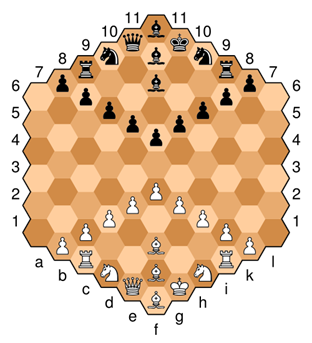
\includegraphics{images/hexStart.png}
    \caption{Startaufstellung Glinski \protect\footnotemark}
    \label{fig:hex:start}
\end{figure}
\footnotetext{\url{https://commons.wikimedia.org/wiki/Category:Glinski\%27s_hexagonal_chess}}

\begin{table}[H]
    \centering
    \begin{tabular}{|c|c|}
        \hline
        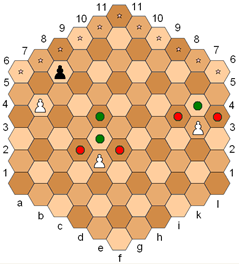
\includegraphics{images/hexPawn.png} & 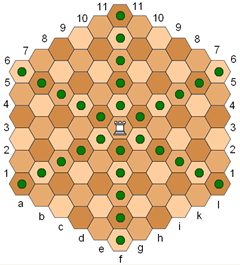
\includegraphics{images/hexRook.png} \\ \hline 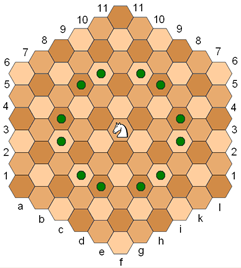
\includegraphics{images/hexKnight.png} & 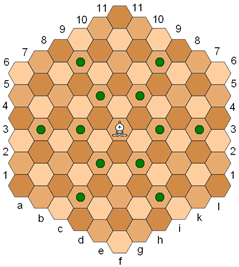
\includegraphics{images/hexBishop.png} \\ \hline 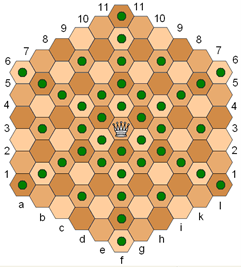
\includegraphics{images/hexQueen.png} & 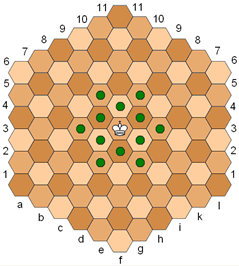
\includegraphics{images/hexKing.png} \\ \hline
    \end{tabular}
    \caption{Gültige Schachzüge in der hexagonalen Variante \protect\footnotemark}
    \label{tab:posMove}
\end{table}
\footnotetext{\url{https://commons.wikimedia.org/wiki/Category:Glinski\%27s_hexagonal_chess}}
\newpage
Der Bauer bleibt weiter die schlechteste Figur des Spiels. Im Vergleich zum normalen Schach gewinnt der Bauer nicht an Zügen und Potential. Am Ende darf der Bauer sich in eine Königin verwandeln. Das macht den Bauern zum Ende des Spiels zu einer wertvollen Figur mit Potential. \cite{GlinskiHexaChess} (vgl. Tabelle \ref{tab:posMove})\par
Der Turm darf sich bis zum Rand in jede Richtung orthogonal bewegen. Spielfiguren behindern seine Bewegungsmöglichkeiten. Der Turm ist die wertvollste Figur nach der Königin. Anders als im normalen Schach ist der Turm allein nicht in der Lage einen König abzuschneiden. Dadurch das der König auch diagonal laufen kann, werden zwei Türme benötigt. Der Turm ist im hexagonalen Schach in der Lage 1/3 des Spielfeldes abzudecken. Im herkömmlichen Schach kann der Turm nur 1/4 von dem Spielfeld abdecken. \cite{GlinskiHexaChess} (vgl. Tabelle \ref{tab:posMove})\par
Das Pferd kann sich auf die Felder bewegen, welche zwei Felder orthogonal entfernt sind und danach jeweils links und rechts oben von der Ausgangsposition. Drei Zügen werden gebraucht, um komplett über das Feld zu kommen. Das Pferd hat sich im Vergleich zum normalen Schach nicht verbessert. \cite{GlinskiHexaChess} (vgl. Tabelle \ref{tab:posMove})\par
Der Bischof bewegt sich diagonal bis zum Ende des Feldes. Der Bischof deckt im hexagonalen Schach 1/7 des Spielfeldes ab. Im normalen Schach wird optimalerweise 1/5 vom Bischof abgedeckt. Drei Bischöfe werden im hexagonalen Schach gebraucht, um den König abzuschneiden. Normalerweise werden dafür nur zwei Bischöfe gebraucht. Im Vergleich der beiden Versionen hat der Bischof an Macht verloren. \cite{GlinskiHexaChess} (vgl. Tabelle \ref{tab:posMove})\par
Die Königin ist weiter die stärkste Figur auf dem Feld. Sie kann sich orthogonal und diagonal bis zum Ende des Feldes bewegen. Dadurch kann die Königin in einem Radius von zwei Feldern alles schlagen. Das ist ein Feld besser als im normalen Schach. Die Königin kann allein den König in Schachmatt stellen, sofern er in eine Ecke gedrängt wird. Ungefähr die Hälfte des Feldes kann die Königin in optimaler Position abdecken. Ein bisschen weniger kann die Königin im normalen Schach abdecken. Weiter noch ist sie nie in der Lage den König allein in ein Schachmatt zu stellen. \cite{GlinskiHexaChess} (vgl. Tabelle \ref{tab:posMove})\par
Der König gewinnt in der Abwandlung an Macht. Er kann sich ein Feld diagonal und orthogonal bewegen. Dadurch werden mehr Türme und Bischöfe gebraucht, um den König auf eine Seite auszugrenzen. Dazu hat der König im hexagonalen Schach vier weitere Bewegungsmöglichkeiten. \cite{GlinskiHexaChess} (vgl. Tabelle \ref{tab:posMove})

    \newcommand{\code}[1]{\texttt{#1}}

\chapter{Implementieren des hexagonalen Schachs nach Glinski}
Für die Implementierung des hexagonalen Schachs wird die Bibliothek \textit{pygame} genutzt. Diese vereinfacht es Spiele zu programmieren. Die Bibliothek stellt Methoden zur Verfügung, welche Fenster erstellen und Objekte malen. So eine Bibliothek erleichtert die Arbeit und ermöglicht einen schnelleren Start mit dem eigentlichen Programm. \textit{pygame} wird als Grundbaustein der Spieleprogrammierung in Python genutzt.

\begin{figure}[H]
    \centering
    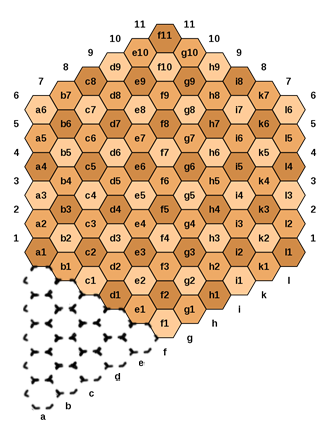
\includegraphics{images/hexIndex.png}
    \caption{Beschriftetes Spielfeld \protect\footnotemark}
    \label{fig:hex:index}
\end{figure}
\footnotetext{\url{https://commons.wikimedia.org/wiki/Category:Glinski\%27s_hexagonal_chess}}

Das Feld besteht aus 91 Hexagonen. Die Hexagone werden in einer zweidimensionalen Liste gespeichert. Mit dem ersten Index wird auf die Reihe, mit dem zweiten Index wird auf die Spalte zugegriffen. Mit den Indizes [0][0] wird das Feld  a6 angesprochen. Das nächste Feld in der Reihe ist bei b7 und wird mit den Indizes [0][1] angesprochen. Die Spalten a,b,c,d und e werden sobald sie kein Feld mehr enthalten mit \textit{None} aufgefüllt, damit die Formatierung der Felder bleibt.\par
Das Hexagon ist eine eigene Klasse. Die Klasse hat die Attribute Stein und Nachbarn. Die Nachbarn sind oben-links, oben, oben-rechts, unten-rechts, unten und unten-links vom Feld. Die Nachbarn sind Referenzen zu den Feldern. Dazu werden die Felder auch noch in einer Liste gespeichert, welche per Index sich in der genannten Reihenfolge aufrufen lassen. Die Nachbarn werden später für das Bewegen der Steine genutzt.\par
Ein Feld wird mit einer selbst geschriebenen Methode markiert. Das Feld wird markiert, wenn ein Feld als Bewegungsmöglichkeit gilt. Ein Feld gilt als mögliches Feld, wenn die Figur nach den Regeln von Glinski sich auf das Feld bewegen darf. Die Methode zum Markieren eines Feldes sieht wie folgt aus.

\begin{lstlisting}[language=python,caption={Felder markieren},captionpos=b,label={lst:hexa:markieren},numbers=left,frame=none,escapechar=|]
def mark_tile(self, tile):
  if not isinstance(tile, GameBoard.Hexagon):|\label{m:line2}|
    return None

  if tile.piece is not None:
    if tile.piece.white is self.white:
      return "taken"

    GameBoard.Hexagon(tile.screen, tile.outer_radius, tile.inner_radius,tile.x_pos, tile.y_pos, (255, 0, 0))|\label{m:line9}|
    tile.piece.move_towards(tile.x_pos, tile.y_pos, False, False)
    tile.is_destination = True
    return "enemy"
  
  GameBoard.Hexagon(tile.screen, tile.outer_radius, tile.inner_radius, tile.x_pos, tile.y_pos, (249, 215, 28))|\label{m:line14}|
  tile.is_destination = True
  return "field can be destination"
\end{lstlisting}

Die Methoden nimmt als Parameter ein Feld an. Wenn der Parameter kein Hexagon ist, was in Zeile \ref{m:line2} abgefragt wird, wird \textit{None} zurückgegeben. Mit \code{if tile.piece is not None:} wird überprüft ob auf dem Feld ein Stein steht. In der If-Abfrage wird weiter abgefragt, ob der Stein die gleiche Farbe hat wie die Figur, mit welcher gespielt wird. Ist das der Fall, wird „taken“ zurückgegeben. Ist auch das nicht der Fall, geht das Programm weiter und kommt zu dem Teil wo das Feld markiert wird. Zeile \ref{m:line9} erstellt ein rotes Hexagon auf der Position, wo das valide Feld liegt. Es muss ein neues Hexagon gemalt werden, da von dem alten nicht die Farbe geändert werden kann. Die Figur, die auf dem Feld stand, wird in diesem Prozess ebenfalls übermalt. Deswegen muss diese wieder in den Vordergrund bewegt werden. Das wird mit \code{tile.piece.move\_towards(tile.x\_pos, tile.y\_pos, False)} gemacht. Als letztes wird die Variable \textit{is\_destination} auf \textit{True} gesetzt. Diese Variable wird beim Klicken auf ein Feld abgefragt. Ist \textit{is\_destination True} wird der Stein auf das Feld bewegt, ist \textit{is\_destination False} passiert nichts. Am Ende des Rumpfes der If-Abfrage wird „enemy“ zurückgegeben. Nach der If-Abfrage folgen die Befehle, welche ausgeführt werden, wenn kein Stein auf dem Feld ist. Es wird ein gelbes, hexagonales Feld in Zeile \ref{m:line14} erstellt. Dadurch werden Felder mit Gegnern und freie Felder unterschieden. Ebenfalls wird die Variable \textit{is\_destination} auf \textit{True} gesetzt. Der Rückgabewert ist „field can be destination“.

\begin{lstlisting}[language=python,caption={Markierung aufheben},captionpos=b,label={lst:hexa:aufheben},numbers=left,frame=none,escapechar=|]
def tile_remove_mark(self, tile):
  if not isinstance(tile, GameBoard.Hexagon): |\label{yes,label}|
    return None

    GameBoard.Hexagon(tile.screen, tile.outer_radius, tile.inner_radius,tile.x_pos, tile.y_pos)
    if tile.piece is not None:
        tile.piece.move_towards(tile.x_pos, tile.y_pos, True, False)
        
    tile.is_destination = False
\end{lstlisting}

\textit{tile\_remove\_mark} entfernt die Markierung wieder. Damit keine Fehler auftreten wird in Zeile \ref{yes,label} erst geprüft, ob der Parameter \textit{tile} wirklich ein Hexagon ist. Danach malt Zeile \ref{r:line5} das Hexagon mit der Standartfarbe. Wenn auf dem Feld eine Figur war, wird diese wieder nach vorne bewegt. Als letztes wird \textit{is\_destination} wieder auf den Standartwert gesetzt.

Die Methode, welche die Figuren bewegt, ist ebenfalls eine eigene Methode. Jede Figur vererbt die Methode von der Elternklasse \textit{Piece}.

\begin{lstlisting}[language=python,caption={Figur bewegen},captionpos=b,label={lst:hexa:bewegen},numbers=left,frame=none,escapechar=|]
def move_towards(self, x, y, replace_bottom=True, moved=True):
    self.rect.x = x + self.offset[0]
    self.rect.y = y + self.offset[1]
    if replace_bottom:
        GameBoard.Hexagon(self.starting_tile.screen, self.starting_tile.outer_radius, self.starting_tile.inner_radius, self.starting_tile.x_pos, self.starting_tile.y_pos) 
        self.screen.blit(self.image, (self.rect.x, self.rect.y))
    pygame.display.flip()
    if moved:
        self.at_start = False

\end{lstlisting}

Die erwarteten Parameter sind die neuen X- und Y-Koordinaten, auf welchen die Figur gemalt wird. Die Standartparameter \textit{replace\_bottom} und \textit{moved} sind ohne Zuweisen beim Methodenaufruf jeweils \textit{False}. In den ersten beiden Zeilen der Methode werden die Koordinaten erneuert. Die Liste \textit{offset} ist ein statischer Wert, welcher die Figur auf das Feld zentriert. Beim Bewegen wird die alte Figur nicht entfernt. Der beste Weg die alte Figur zu entfernen, ist ein neues Hexagon über die alte Figur zu malen. \code{pygame.display.flip()} updatet das Fenster und die Änderungen werden angezeigt. Als letztes wird in der Methode die Variable \textit{at\_start} gleich \textit{False} gesetzt. \textit{at\_start} ist wichtig für die Steine, welche als erste Bewegungsmöglichkeiten besondere Regeln haben.\par
Die Figuren haben jeweils zwei Methoden, welche von der Elternklasse vererbt werden. Beim Klicken auf eine Figur wird die \textit{show\_moves} Methode aufgerufen. Jede Figur hat eine eigene \textit{show\_moves} Methode, welche alle Felder mithilfe der \textit{mark\_tile} Methode markiert.\par
Für die Figur werden die Seiten mit einer Schleife durchgelaufen. Als Beispiel wird der Turm genommen. Das Prinzip lässt sich auf die anderen Figuren übertragen. Bauern haben extra Regeln, welche sich aber aus dem Verhalten vom Turm ableiten lassen.

\begin{lstlisting}[language=python,caption={Figur zeige Bewegungsmöglichkeiten},captionpos=b,label={lst:hexa:show},numbers=left,frame=none,escapechar=|]
def show_moves(self):
    self.rows = [[], [], [], [], [], []]
    for i in range(len(self.starting_tile.sides)):
        tile = self.starting_tile.sides[i]
        while mark_tile(self, tile) is not None:
            self.rows[i].append(tile)
            if tile.piece is not None:
                break
            tile = tile.sides[i]

\end{lstlisting}

Mit der \textit{for}-Schleife werden die einzelnen Seiten durchgelaufen. Die Seite wird per Index bestimmt. Eine \textit{while}-Schleife läuft solange durch bis \textit{mark\_tile None} zurück gibt. Der Vorteil davon, ist dass das Feld direkt mit gefärbt wird. In der \textit{while}-Schleife werden die Felder an eine Liste angehängt. Beim Löschen der Markierung werden die Felder von der Liste durchgelaufen. Wenn die Schleife auf einen Spielstein trifft gibt \textit{mark\_tile} kein \textit{None} zurück. Deswegen muss die \textit{while}-Schleife unterbrochen werden, wenn auf einen Stein getroffen wird. Als letztes wird die Variable \textit{tile} zu dem passenden Nachbarn aktualisiert.\par
In dem \textit{main.py} werden die wechselnden Spielzüge verwaltet. Eine \textit{while}-Schleife läuft solange durch, bis das Fenster geschlossen wird oder ein König geschlagen wird. Ein Klick auf ein Feld wird wahrgenommen, indem die Distanz von jedem Feld zur Maus gemessen wird, sobald eine Taste gedrückt wird. Wenn die Distanz kleiner ist als ein \textit{treshhold} werden die möglichen Züge gezeigt. Wird ein valides Feld ausgewählt, bewegt sich die Figur zu dem Feld und der andere Spieler ist an der Reihe. Wenn ein Feld ausgewählt wird, was als nicht valide gilt, wird die Auswahl für die Figur aufgehoben und eine neue Figur kann ausgewählt werden.\par
Ein Problem bei der jetzigen Implementierung ist, dass Züge auch valide sind, wenn der König im Schach steht oder dadurch im Schach stehen würde. Durch die vielen Möglichkeiten, wie ein König im Schach stehen kann, wurde auf eine Implementierung des Features verzichtet und der Spieler muss jetzt selber auf seinen König aufpassen.

    \chapter{Zusammenfassung}

Im Vergleich der beiden Programmiersprache gibt es keinen klaren Sieger. Python ist eine vergleichsweise langsame Programmiersprache, weil sie interpretiert wird und Java kompiliert. Programme, die nicht auf Laufzeit optimiert werden müssen, können also in Python geschrieben werden. Python ist wegen der Syntax intuitiver. Durch wenig Code lässt sich schon schnell ein Programm programmieren. Die Bibliotheken helfen umso mehr. Ein Programm, welches viele Prozesse schnell ausführen soll, sollte auf jeden Fall in Java geschrieben werden. Bis ein Resultat erzielt wird dauert es vergleichsweise länger, lohnt sich jedoch. Java und Python funktionieren auf jeder Plattform, was die Wahl einer Programmiersprache nicht auf Plattformen beschränkt.\par
Welche Programmiersprache man lernen sollte hängt von zwei Faktoren ab. Wenn schnell Erfolge erzielt werden sollen, ist Python zu empfehlen. Ist der Hintergedanke ein tiefgründiges Verständnis vom Programmieren ist Java eher die Wahl. Optimal ist ein Mix aus den beiden Programmiersprachen. Mit Python sollte angefangen werden, um ein generelles Grundverständnis zu erlangen und Motivation für das Programmieren und die Informatik zu gewinnen. Danach Java für einen tieferen Einblick in die Prinzipien und Prozesse.\par
Diese Aufteilung lässt sich auch auf die Schule anwenden. Schüler sind motivierter, wenn sie schnell Ergebnisse erzielen und nicht erst das Grundgerüst aufbauen müssen. Von den Klassen sieben bis neun sollte Python gelehrt werden. Für die Oberstufe wird dann auf Java oder eine ähnliche Programmiersprache, wie C, C++ oder C\# gewechselt. Wenn die Schüler in der zehnten Klasse einen Einblick auf die Q1 und Q2 bekommen, können sie sich dann festlegen, ob sie Informatik weiterwählen oder bei einem Grundverständnis bleiben.
\par
Im Hinblick auf die zweite Leitfrage dieser Facharbeit, welche Schachvariante besser ist, lässt sich ähnlich wie bei den Programmiersprachen argumentieren. Meiner Meinung nach ist die hexagonale Variante besser. Es werden viele neue Möglichkeiten durch die zwei weiteren Seiten eröffnet. Dennoch empfehle ich nicht mit hexagonalem Schach in das Thema Schach einzusteigen. Besonders, weil das Vorhersagen und Planen von Zügen schwieriger ist. Ein erfahrener Spieler sollte sich die hexagonale Variante aber nicht entgehen lassen.

    
    \appendix
    \pagestyle{scrplain}
    \listoffigures
    \listoftables
    %\clearpage \phantomsection 
    %\addcontentsline{toc}{chapter}{Algorithmenverzeichnis}
    %\listofalgorithmes
    \renewcommand*{\lstlistlistingname}{Listingsverzeichnis}
    \lstlistoflistings
    \flushbottom
    \bibliographystyle{babunsrt-fl}
    \bibliography{literature/literature}
    \KOMAoptions{open=right} % Plaziert Kapitel wieder nur auf rechten Seiten
    \textbf{Hinweis zu den Quellenangaben:} \par
    „...“[x] - direktes Zitat \par
    ...[x].  - Quellenangabe bezieht sich auf den Satz \par
    .[x]     - Quellenangabe bezieht sich auf den gesamten Absatz
    \chapter{Quicksort in Python}
\lstinputlisting[language=python,numbers=left]{code/quicksort.py}
\label{quicksort:pyton}
\chapter{Quicksort in Java}
\label{quicksort:java}
\lstinputlisting[language=java]{code/quicksort.java}

\end{document}
